\documentclass[tikz,border=2pt]{standalone}
\usepackage{amsmath,amssymb}
\usetikzlibrary{arrows.meta,calc}
\begin{document}
% Histories of the twice-repeated prisoner's dilemma (stages t = 0, 1): h^0 is empty; the four stage-0 action
% profiles give the four histories h^1 = (C,C), (C,D), (D,C), (D,D); each of the 1 + 4 = 5
% non-terminal histories starts a subgame (shaded: the 4 proper subgames).
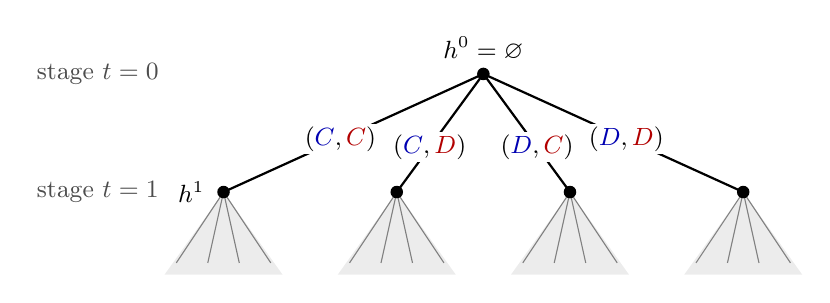
\begin{tikzpicture}[font=\small, >={Latex[length=2mm]},
    dec/.style={circle, fill, inner sep=1.6pt}]
  \def\C{\textcolor{blue!70!black}{C}} \def\D{\textcolor{blue!70!black}{D}}
  \def\c{\textcolor{red!70!black}{C}} \def\d{\textcolor{red!70!black}{D}}
  % proper subgames
  \foreach \x in {-3.3,-1.1,1.1,3.3}
    \fill[gray!15] (\x,-1.5) -- (\x-0.75,-2.55) -- (\x+0.75,-2.55) -- cycle;
  % stage 1
  \foreach \x in {-3.3,-1.1,1.1,3.3}
    \draw[thick] (0,0) -- (\x,-1.5);
  \foreach \x/\a/\b/\p in {-3.3/\C/\c/0.55, -1.1/\C/\d/0.62, 1.1/\D/\c/0.62, 3.3/\D/\d/0.55}
    \node[fill=white, inner sep=1pt] at ($(0,0)!\p!(\x,-1.5)$) {$(\a,\b)$};
  % stage 2: four action profiles after each history
  \foreach \x in {-3.3,-1.1,1.1,3.3} {
    \foreach \dx in {-0.6,-0.2,0.2,0.6}
      \draw[gray] (\x,-1.5) -- (\x+\dx,-2.4);
    \node[dec] at (\x,-1.5) {};
  }
  \node[dec] at (0,0) {};
  % labels
  \node[anchor=south] at (0,0.05) {$h^0=\varnothing$};
  \node[anchor=east] at (-3.42,-1.5) {$h^1$};
  \node[anchor=east, gray!60!black] at (-4.0,0) {stage $t=0$};
  \node[anchor=east, gray!60!black] at (-4.0,-1.5) {stage $t=1$};
\end{tikzpicture}
\end{document}
